\chapter{Photodetection and Photon Counting: Why We Count n(n-1)}
\label{chap:e07}

\begin{chapteropening}
Up to the previous chapter, we had ``read'' light very thoroughly: light is a set of mode excitations, every mode is a harmonic oscillator, a photon is one portion of energy in a mode, and the number, coherent, and thermal states (even at the same brightness) have utterly different tendencies \(b_2\) for photons to arrive in pairs (Chapter~\ref{chap:e06}). But all of this still stayed on the ``light state'' side. What the telescope side hands back is never a wave function, but a string of cold clicks: at some moment, at some pixel, a snap. What this chapter builds is precisely the bridge between these two sides: how exactly does a light state become a string of counts on a detector? We will work out three things step by step. First, why ``detecting one photon,'' mathematically, forces us to count \(n(n-1)\) rather than \(n^2\): that subtracted \(n\) is precisely ``the same photon cannot pair with itself.'' Second, how to slice an event table into time gates and, with a number called the Mandel \(Q\), see at a glance whether this beam of light ``clusters'' more than Poisson or is more ``orderly.'' Third, why the majestic \(g^{(2)}(0)=2\) of the textbooks shrinks, on a real telescope, into a small number like \(1+10^{-3}\) or even \(1+10^{-6}\): not that the signal is gone, but that it has been diluted by thousands upon thousands of modes. By the end of this chapter, you will hold the full conversion from ``the quantum state of light'' to ``count statistics that can truly be taken and fitted.''
\end{chapteropening}

\section{Where Clicks Come From: Detection Is Absorbing One Photon}
\label{sec:e07-absorption}

Let us return to the plainest question: when a detector ``sees'' one photon, what physically happens?

It is not that a photon hits a wall and bounces back, nor that it is ``caught'' like a little ball. Real photodetection is an \emph{absorption}: one portion of energy in the light field is handed to the detector (knocking out a photoelectron, triggering an avalanche, flipping a pixel), and at the same time \textbf{the light field has one photon fewer}. In Chapter~\ref{chap:e05} we already stressed this sentence repeatedly and wrote it in operator language: absorption uses only the positive-frequency field operator \(\hat E^{(+)}\), because \(\hat E^{(+)}\) carries the annihilation operator \(\hat a\) (removing one photon), not the creation operator \(\hat a^\dagger\).

Now fix attention on a single mode. Here the positive-frequency field is proportional to that mode's annihilation operator, \(\hat E^{(+)}\propto\hat a\). Quantum detection theory (Glauber) tells us a clean rule: \textbf{the probability of a detector ``snapping'' at some instant is proportional to the annihilation operator sandwiched and averaged in the light state.} One click corresponds to one absorption, so the single-click rate is proportional to

\begin{equation}
  p_1\ \propto\ \big\langle\,\hat E^{(-)}\hat E^{(+)}\,\big\rangle
  \ \propto\ \big\langle\,\hat a^\dagger\hat a\,\big\rangle
  =\langle\hat n\rangle .
  \label{eq:e07-single-click}
\end{equation}
\begin{formulaexplain}
The single-click probability is proportional to \(\langle\hat a^\dagger\hat a\rangle=\langle\hat n\rangle\). \(\hat a\) acts first (absorbing that one photon), and \(\hat a^\dagger\) is its Hermitian conjugate; sandwiched and averaged, this is ``how many photons there are on average.'' In one sentence: \emph{the click rate follows the photon number}.
\end{formulaexplain}

Let us account for each symbol. \(\hat E^{(+)}\), \(\hat E^{(-)}=[\hat E^{(+)}]^\dagger\) are the positive- and negative-frequency field operators (Chapter~\ref{chap:e05}); in the single mode they are respectively proportional to \(\hat a\) and \(\hat a^\dagger\), both dimensionless (the proportionality constant is absorbed into the detection efficiency). \(\hat n=\hat a^\dagger\hat a\) is the photon-number operator, with eigenvalues \(N=0,1,2,\dots\), pure integers with no units. The angle brackets \(\langle\cdot\rangle\) denote the quantum expectation over the light state. The physical meaning of \eqref{eq:e07-single-click} could not be plainer: to make the detector snap more, one must make the average photon number in the mode larger. This is also why, in Chapter~\ref{chap:e05}, ``every mode is actually quite dim'' (\(\bar n_\nu\sim10^{-2}\)) directly translates into ``the click rate of a single mode is actually quite low.''

\paragraph{Two coincident clicks: normal ordering automatically subtracts ``pairing with itself''}
\label{sec:e07-normal-ordering}

What is truly interesting is two clicks. Suppose the question is no longer ``the probability of one snap,'' but ``the probability of \emph{two} snaps at (almost) the same instant''; this is precisely the core quantity of Hanbury Brown--Twiss intensity interferometry, coincidence counting, and second-order coherence measurement. Two clicks mean two absorptions: the light field \emph{successively} loses two photons. By the same detection rule, lining up two \(\hat E^{(+)}\), the two-coincident-click rate is proportional to

\begin{equation}
  p_2\ \propto\ \big\langle\,\hat E^{(-)}\hat E^{(-)}\hat E^{(+)}\hat E^{(+)}\,\big\rangle
  \ \propto\ \big\langle\,\hat a^\dagger\hat a^\dagger\hat a\,\hat a\,\big\rangle .
  \label{eq:e07-two-click}
\end{equation}
\begin{formulaexplain}
The two-coincident-click probability is proportional to \(\langle\hat a^\dagger\hat a^\dagger\hat a\hat a\rangle\): all annihilation operators (absorption) lined up on the right, all creation operators on the left. This arrangement of ``creation on the left, annihilation on the right'' is called \textbf{normal ordering}, and it is precisely the mathematical embodiment of ``two clicks correspond to two real absorptions.''
\end{formulaexplain}

Note the order of operators in \eqref{eq:e07-two-click}: the two \(\hat a\) (absorption) sit adjacent on the far right, the two \(\hat a^\dagger\) on the far left. This arrangement of ``annihilation all on the right, creation all on the left'' is called normal ordering. It is not an artificial convention but is imposed by the physics of detection: the detector responds only to \emph{genuinely absorbed} photons, so each click corresponds to one \(\hat a\) acting on the state, and two clicks act two \(\hat a\) on it in succession.

Now we reach the key point of the question in this chapter's title. What exactly does the operator combination \(\hat a^\dagger\hat a^\dagger\hat a\hat a\) in \eqref{eq:e07-two-click} equal? We do not guess; we directly use the \emph{one} algebraic fact used repeatedly in Chapter~\ref{chap:e05} (the commutation relation \([\hat a,\hat a^\dagger]=1\), that is, \(\hat a\hat a^\dagger=\hat a^\dagger\hat a+1\)) to work it open step by step. The goal is to write it as a function of the number operator \(\hat n=\hat a^\dagger\hat a\).

First look at the square of the number operator:
\[
  \hat n^2=(\hat a^\dagger\hat a)(\hat a^\dagger\hat a)
  =\hat a^\dagger\,\underbrace{(\hat a\,\hat a^\dagger)}_{=\,\hat a^\dagger\hat a+1}\,\hat a
  =\hat a^\dagger(\hat a^\dagger\hat a+1)\hat a
  =\hat a^\dagger\hat a^\dagger\hat a\,\hat a+\hat a^\dagger\hat a .
\]
That middle step is replacing \(\hat a\hat a^\dagger\) with \(\hat a^\dagger\hat a+1\), the only non-trivial algebra used in the whole derivation. Recognizing the second term on the right as \(\hat n\), rearranging gives the bridge between normal ordering and the number operator:
\begin{equation}
  \hat a^\dagger\hat a^\dagger\hat a\,\hat a
  =\hat n^2-\hat n
  =\hat n(\hat n-1).
  \label{eq:e07-normal-identity}
\end{equation}
\begin{formulaexplain}
The normal-ordered two-photon operator \emph{exactly} equals \(\hat n(\hat n-1)\). If the mode has \(N\) photons, the ``ordered photon pairs'' that can be formed number \(N^2\), but \(N\) of those are ``the same photon paired with itself''; normal ordering automatically subtracts these \(N\) spurious pairs, leaving \(N(N-1)\) \emph{true} pairs.
\end{formulaexplain}

This line is worth stopping to savor. It says: \textbf{normal ordering = automatically subtracting self-pairing.} Imagine that at some instant the mode has exactly \(N\) photons. If, without thinking, one pairs ``the first photon counted'' and ``the second photon counted'' at will, there are \(N\times N=N^2\) \emph{ordered} choices in all. But \(N\) of those are ``the first and second counted are the \emph{same} photon,'' which is physically impossible, because one coincidence detection needs a START pulse and a STOP pulse, and they must come from \emph{two different absorptions}; once the same photon is absorbed it is gone and can never trigger a second snap. So the number of ordered photon pairs actually available is \(N(N-1)=N^2-N\), and that subtracted \(N\) is precisely the self-pairing. The term \(\hat n\) by which \(\hat n^2\) and \(\hat n(\hat n-1)\) differ in \eqref{eq:e07-normal-identity}, not one symbol more nor one fewer, is exactly these self-pairings.

This is also the origin of that pair factor \(b_2\) of Chapter~\ref{chap:e06}. Recall that there we defined the single-mode zero-delay pairing tendency as
\[
  b_2\equiv\frac{\langle\hat n(\hat n-1)\rangle}{\langle\hat n\rangle^2},
\]
and computed the number state to give \(b_2=1-1/n\) (antibunching), the coherent state \(b_2=1\) (Poisson baseline), the thermal state \(b_2=2\) (bunching). Now we finally understand: the \(\langle\hat n(\hat n-1)\rangle\) in the numerator is not some odd thing defined off the top of someone's head, but the inevitable result of the detector \emph{physically being able to count only true pairs}. Normalizing \eqref{eq:e07-single-click} and \eqref{eq:e07-two-click} gives

\begin{equation}
  \frac{p_2}{p_1^2}\ \propto\
  \frac{\langle\hat a^\dagger\hat a^\dagger\hat a\hat a\rangle}{\langle\hat a^\dagger\hat a\rangle^2}
  =\frac{\langle\hat n(\hat n-1)\rangle}{\langle\hat n\rangle^2}
  =b_2 .
  \label{eq:e07-b2-from-clicks}
\end{equation}
\begin{formulaexplain}
Dividing the probability of ``two snaps together'' by the probability of ``two independent single snaps'' gives the pair factor \(b_2\). It is the quantity the detector measures: \(b_2>1\) photons like to cluster (bunching), \(b_2<1\) photons avoid each other (antibunching), \(b_2=1\) each comes on its own (Poisson).
\end{formulaexplain}

One sentence to close this section: \textbf{what the detector counts is always the correlation between ``different absorption events,'' that is, \(\langle n(n-1)\rangle\), not a continuous waveform, nor \(\langle n^2\rangle\).} Normal ordering is not a formalist trick; it is the hardest physical fact that ``a photon can be absorbed only once.'' Figure~\ref{fig:e07-factorial-moments} draws this out: the same counting distribution, weighted by \(N^2\) versus weighted by \(N(N-1)\), differs by exactly that self-pairing diagonal.

\begin{figure}[tbp]
\centering
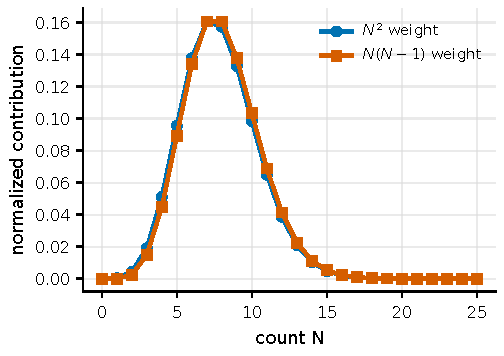
\includegraphics[width=0.86\linewidth]{figures/generated/chapter_04/ch04_factorial_moments.pdf}
\caption{The ordinary second moment \(N^2\) and the factorial moment \(N(N-1)\) weight different photon numbers \(N\) differently. Coincidence detection concerns only ordered pairs formed of \emph{different} photons, so normal ordering automatically subtracts the spurious contribution \(N^2-N(N-1)=N\) of ``the same photon paired with itself.'' This is exactly why what appears in second-order photon statistics is \(\langle N(N-1)\rangle\), not \(\langle N^2\rangle\).}
\label{fig:e07-factorial-moments}
\end{figure}

\section{Slicing the Event Table into Time Gates: Mean, Variance, and the Mandel Parameter}
\label{sec:e07-time-gate}

The previous section discussed ``instantaneous'' operator expectations. But what a real telescope hands back is a time-stamped event table: a long string of records of ``some photon arriving at some moment'' (the structure, clock, dead time, and other hardware details of this table are left for Chapter~\ref{chap:e13}). To turn an operator expectation like \eqref{eq:e07-b2-from-clicks} into a number that can truly be computed from data, we need a concrete operation: \textbf{slice continuous time into ``time gates'' (bins) each of width \(\Delta t\), and count how many photons fall into each.}

Let the count in the \(k\)th time gate be \(N_k\) (a dimensionless integer). Collecting the counts of many gates gives a counting distribution \(P(N)\): what fraction of time gates have \(N\) photons. For this distribution, we care about the two most basic statistics, the mean and the variance:

\begin{equation}
  \bar N=\langle N\rangle=\sum_{N=0}^{\infty}N\,P(N),
  \qquad
  \sigma_N^2=\big\langle N^2\big\rangle-\bar N^{\,2}
  =\sum_{N=0}^{\infty}(N-\bar N)^2\,P(N).
  \label{eq:e07-mean-var}
\end{equation}
\begin{formulaexplain}
\(\bar N\) is the \emph{mean} count per time gate, and \(\sigma_N^2\) is the size of the \emph{fluctuation} of the count between gates (the variance). The mean tells you ``how bright on average,'' the variance tells you ``how much it flickers.'' Judging the quantumness of light looks at the latter relative to the former.
\end{formulaexplain}

Let us account for each: \(\bar N\) is dimensionless, the mean photon number within the gate width \(\Delta t\), equal to the count rate \(r\) (units \(\mathrm{s^{-1}}\)) times the gate width, \(\bar N=r\,\Delta t\). \(\sigma_N^2\) is also dimensionless, the average of the squared deviation of the count from the mean. Here one must remember something very counterintuitive in astronomy: the gate width \(\Delta t\) is usually chosen very small, say \(\Delta t=1\,\mathrm{ns}\), while the count rate of a visible-light point source may be only \(r=10^6\,\mathrm{s^{-1}}\), so

\[
  \bar N=r\,\Delta t=(10^6\,\mathrm{s^{-1}})(10^{-9}\,\mathrm{s})=10^{-3}.
\]

That is, \emph{only about one in a thousand time gates holds a photon}, the vast majority of gates are empty (\(N=0\)), occasionally a gate has \(N=1\), and the chance of two photons in the same gate is as small as \(\sim10^{-6}\). Intensity-correlation signals are never read out from a ``light-curve fluctuation'' visible to the naked eye, but are accumulated bit by bit from the tiny statistical deviations of \(10^8\) or \(10^{12}\) time gates. This is also why we must use statistics, not the eye, to judge the properties of light.

\paragraph{Taking Poisson as the zero point: Mandel Q}
\label{sec:e07-mandel-q}

Now we need a ruler to measure ``whether this beam of light clusters more than random arrival, or is more orderly.'' The natural zero point is the \textbf{Poisson distribution}: if photons each come on their own, mutually independent (a coherent state is exactly so, see Chapter~\ref{chap:e06}), the count follows Poisson statistics, which has a signature property, the \emph{variance is exactly equal to the mean}:
\[
  \text{Poisson:}\quad \sigma_N^2=\bar N .
\]
(We computed this directly from \(P(N)=e^{-\bar N}\bar N^N/N!\) in Chapter~\ref{chap:e06}; it is the definition of shot noise.) Taking this as the zero point, Mandel uses a dimensionless number, the \textbf{Mandel parameter} (Mandel \(Q\) parameter), to measure the deviation:

\begin{equation}
  Q\equiv\frac{\sigma_N^2-\bar N}{\bar N}.
  \label{eq:e07-mandel-q}
\end{equation}
\begin{formulaexplain}
\(Q\) sets the Poisson \(\sigma_N^2=\bar N\) as the zero point and measures ``by what fraction the variance exceeds (or falls short of) the mean.'' \(Q=0\) Poisson (coherent state), \(Q>0\) super-Poisson, photons cluster (thermal light), \(Q<0\) sub-Poisson, photons overly regular (can only be non-classical light).
\end{formulaexplain}

Read term by term. The numerator \(\sigma_N^2-\bar N\) is ``the part by which the variance exceeds Poisson,'' and the denominator \(\bar N\) makes it dimensionless. Three cases, three physics:

\begin{itemize}
  \item \textbf{\(Q=0\) (Poissonian)}: the variance exactly equals the mean. Photons arrive independently at random, with no extra clustering and no extra regularity. An ideal stable laser, a coherent state, is here.
  \item \textbf{\(Q>0\) (super-Poissonian)}: the variance is larger than the mean. Photons tend to arrive \emph{in groups}: some stretch of time has excess intensity and multiple photons crowd in; another stretch is low and they thin out together. This is the signature of thermal light and chaotic light, and the source of HBT bunching.
  \item \textbf{\(Q<0\) (sub-Poissonian)}: the variance is \emph{smaller} than the mean, the count more ``regular,'' more evenly spaced than the random case. This cannot be explained by any positive classical intensity fluctuation and is a genuine non-classical signal (single-photon source, resonance fluorescence). Note \(Q\) has a lower bound: because \(N\ge0\), one can prove \(Q\ge-1\), with \(Q=-1\) corresponding to an ideal number state with completely fixed photon number in every gate.
\end{itemize}

An order-of-magnitude example. The count of single-mode thermal light within gate width \(\Delta t\) follows the Bose--Einstein distribution, with variance \(\sigma_N^2=\bar N+\bar N^2\) (Chapter~\ref{chap:e06}). Substituting into \eqref{eq:e07-mandel-q}:
\[
  Q_{\rm th}=\frac{(\bar N+\bar N^2)-\bar N}{\bar N}=\bar N .
\]
The \(Q\) of ideal single-mode thermal light equals its own mean count, which sounds substantial, but do not forget that in the visible few-photon-per-mode limit \(\bar n_\nu\sim10^{-2}\) (Chapter~\ref{chap:e05}), so even for pure single-mode thermal light, \(Q\) itself is only a few percent. Real multi-mode observation presses it even lower, which is precisely the theme of the next section.

\section{From Mandel Q to g(2)(0): An Algebraic Identity}
\label{sec:e07-q-to-g2}

We now have two languages: one is the language of ``photons arriving in pairs,'' whose protagonist is \(g^{(2)}(0)=\langle N(N-1)\rangle/\bar N^2\) (which is the time-gate version of the previous chapter's \(b_2\), and also the value of the second-order coherence function of Chapter~\ref{chap:e08} at zero delay); the other is the language of ``count variance,'' whose protagonist is the Mandel \(Q\). These two say the same thing, and what \emph{precisely} connects them is only a piece of middle-school algebra.

The key step is to express the factorial moment \(\langle N(N-1)\rangle\) in terms of the mean and the variance. Expand \(N(N-1)=N^2-N\), and average both sides:
\[
  \big\langle N(N-1)\big\rangle=\big\langle N^2\big\rangle-\langle N\rangle
  =\big\langle N^2\big\rangle-\bar N .
\]
Then use the definition of the variance \(\sigma_N^2=\langle N^2\rangle-\bar N^2\), that is, \(\langle N^2\rangle=\sigma_N^2+\bar N^2\), substituting in:
\begin{equation}
  \big\langle N(N-1)\big\rangle=\sigma_N^2+\bar N^{\,2}-\bar N .
  \label{eq:e07-identity}
\end{equation}
\begin{formulaexplain}
A purely algebraic identity: factorial moment = variance + mean squared \(-\) mean. It converts the \(\langle N(N-1)\rangle\) of the ``pair language'' into the \(\sigma_N^2\) and \(\bar N\) of the ``variance language,'' and is the sole bridge connecting \(g^{(2)}(0)\) and \(Q\).
\end{formulaexplain}

There is no physical approximation here; it is purely a matter of splitting \(N(N-1)\) open and rearranging, and it holds for \emph{any} counting distribution. Now substitute it into the definition of \(g^{(2)}(0)\). Dividing by \(\bar N^2\):
\[
  g^{(2)}(0)=\frac{\langle N(N-1)\rangle}{\bar N^{\,2}}
  =\frac{\sigma_N^2+\bar N^{\,2}-\bar N}{\bar N^{\,2}}
  =\underbrace{\frac{\bar N^{\,2}}{\bar N^{\,2}}}_{=1}
  +\frac{\sigma_N^2-\bar N}{\bar N^{\,2}} .
\]
Take one look at the numerator and denominator of the last term: \(\sigma_N^2-\bar N\) is exactly the numerator of the Mandel \(Q\), and \(Q=(\sigma_N^2-\bar N)/\bar N\), so \((\sigma_N^2-\bar N)/\bar N^2=Q/\bar N\). Thus
\begin{equation}
  g^{(2)}(0)=\frac{\langle N(N-1)\rangle}{\bar N^{\,2}}
  =1+\frac{Q}{\bar N}.
  \label{eq:e07-g2-q}
\end{equation}
\begin{formulaexplain}
The zero-delay second-order coherence \(g^{(2)}(0)\) and the Mandel \(Q\) differ only by a \(\bar N\). \(Q\) measures the absolute variance excess, \(g^{(2)}(0)\) measures the normalized pairing excess; the smaller the mean count \(\bar N\), the larger a \(g^{(2)}(0)-1\) the same \(Q\) levers up.
\end{formulaexplain}

Let us account term by term: \(g^{(2)}(0)\) is dimensionless, \(=1\) the independent-arrival baseline, \(>1\) bunching, \(<1\) antibunching. \(Q\) is dimensionless, \(\bar N\) is dimensionless. Equation \eqref{eq:e07-g2-q} is the most practical conversion of this chapter: it locks the ``variance language'' and the ``pair language'' together. Use it to check self-consistency: single-mode thermal light \(Q_{\rm th}=\bar N\), substituting gives \(g^{(2)}(0)=1+\bar N/\bar N=2\), exactly the thermal bunching peak of Chapter~\ref{chap:e06}; coherent state \(Q=0\), giving \(g^{(2)}(0)=1\), the Poisson baseline. Both ends check out.

Equation \eqref{eq:e07-g2-q} also hides a key lesson for astronomical observation, which Figure~\ref{fig:e07-mandel-q-g2} draws out: \(\bar N\) is in the denominator. When the mean count is very low (the weak-light limit), even a very small \(Q\) can correspond to a \(g^{(2)}(0)\) markedly deviating from 1; conversely, widening the time gate makes \(\bar N\) larger and also averages many mutually incoherent time modes into the same \(N\), both together diluting away \(g^{(2)}(0)-1\). So there is an iron rule that must be written into any intensity-correlation report:

\begin{quote}
\textbf{Reporting only \(g^{(2)}(0)\) or only \(Q\) is incomplete.} One must simultaneously give four things: \(Q\) (or \(g^{(2)}(0)-1\)), the \textbf{time gate width \(\Delta t\)}, the \textbf{effective mode count \(M\)}, and the \textbf{mean count \(\bar N\)}. Miss any one, and others cannot judge whether what you measured is an intrinsic signal or a residual shadow after gate-width dilution.
\end{quote}

\begin{figure}[tbp]
\centering
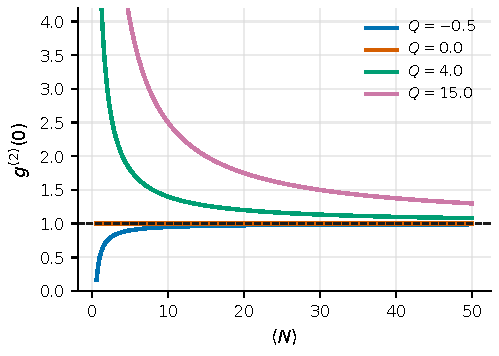
\includegraphics[width=0.86\linewidth]{figures/generated/chapter_04/ch04_mandel_q_g2.pdf}
\caption{Within a fixed time gate, the Mandel \(Q\) determines the zero-delay second-order coherence through \(g^{(2)}(0)=1+Q/\bar N\). The lower the mean count \(\bar N\), the larger the \(g^{(2)}(0)-1\) that the same \(Q\) levers up; widening the time gate or averaging more modes makes \(\bar N\) grow and \(Q\) be diluted, and the curve gradually falls back to the Poisson baseline 1. This explains why, when reporting second-order correlations, one must simultaneously note the gate width, the mode count, and the mean count.}
\label{fig:e07-mandel-q-g2}
\end{figure}

\section{Multi-Mode Dilution: Why the Astronomical Excess Is a Small Number, Not 1}
\label{sec:e07-multimode}

In the textbooks, the bunching peak of single-mode thermal light is a proud \(g^{(2)}(0)=2\), that is, an excess \(g^{(2)}(0)-1=1\). But open any real astronomical intensity-interferometry paper and the peak height you see is a humble small number like \(10^{-3}\) or \(10^{-6}\). Is the signal lost? No. It has been diluted by \emph{multi-mode averaging}. This section works out the dilution.

Recall Chapter~\ref{chap:e05}: in astronomy ``one channel'' is almost never a single quantum mode, but a sum of \(M\) independent modes, \(M\simeq(\Delta t/\tau_c)(A\Omega/\lambda^2)N_{\rm pol}\), readily thousands upon thousands in the visible. Now let us work out the statistical consequence of this sentence.

Let the detected total count \(N\) be the sum of the contributions of \(M\) \emph{independent, similar-intensity} thermal-light modes, each with mean count \(m=\bar N/M\). For a single thermal mode, the variance is \(m+m^2\) (Bose--Einstein, Chapter~\ref{chap:e06}). When independent random variables are added, \textbf{the means add and the variances also add} (this is the standard conclusion in probability theory that the variance of independent variables is additive, which we cite directly). So the total variance is
\[
  \sigma_N^2=\sum_{i=1}^{M}(m+m^2)=M m+M m^2
  =\underbrace{Mm}_{=\bar N}+M\Big(\frac{\bar N}{M}\Big)^2 .
\]
The first term \(Mm=\bar N\) is the total mean (the shot-noise part), and the second term simplifies to \(M\cdot\bar N^2/M^2=\bar N^2/M\). Thus
\begin{equation}
  \sigma_N^2=\bar N+\frac{\bar N^{\,2}}{M}.
  \label{eq:e07-multimode-var}
\end{equation}
\begin{formulaexplain}
After averaging \(M\) independent thermal modes, the two parts of the variance: \(\bar N\) is the unavoidable shot noise, and \(\bar N^2/M\) is the extra ``fluctuation noise'' of thermal light. The more modes (the larger \(M\)), the thinner the second term is spread, and the more the light looks like Poisson.
\end{formulaexplain}

Let us account term by term: \(\bar N\) is the total mean count (dimensionless), \(M\) the effective mode count (dimensionless, \(\ge1\)), and \(\bar N^2/M\) the super-Poisson fluctuation remaining after dilution by \(M\). Now stuff \eqref{eq:e07-multimode-var} into the Mandel \(Q\) and \(g^{(2)}(0)\). First compute \(Q\):
\[
  Q=\frac{\sigma_N^2-\bar N}{\bar N}
  =\frac{\bar N^2/M}{\bar N}=\frac{\bar N}{M}.
\]
Then use the conversion \eqref{eq:e07-g2-q}:
\begin{equation}
  g^{(2)}(0)=1+\frac{Q}{\bar N}=1+\frac{1}{M}.
  \label{eq:e07-multimode-g2}
\end{equation}
\begin{formulaexplain}
After averaging \(M\) independent thermal modes, the bunching peak height drops from the single-mode \(g^{(2)}(0)-1=1\) to \(1/M\). This \(1/M\) law is the root of why the excess is always a small number in astronomical intensity interferometry.
\end{formulaexplain}

This \(g^{(2)}(0)=1+1/M\) is astonishingly clean, and the physics is clear too: the intensity fluctuations of \(M\) independent modes are each random and cancel one another, and on average the intensity grows steadier and steadier, so the ``clustering'' effect of bunching is thinned by a factor of \(M\). \(M=1\) gives the classical 2; \(M=1000\) gives \(1+10^{-3}\); \(M=10^6\) gives \(1+10^{-6}\). This is why what is directly read off an astronomical HBT plot is never the majestic 2, but a small-number excess that must be dug out from a vast number of event pairs.

Where do those \(M\) come from? Count them one by one (all within the mode-counting framework of Chapter~\ref{chap:e05}):

\begin{itemize}
  \item \textbf{Polarization (2 modes)}: if the polarization is not projected onto a single channel, the two orthogonal polarizations are each an independent thermal mode, \(M_{\rm pol}\simeq2\), immediately pressing the ideal peak from 2 down to 1.5.
  \item \textbf{Spatial speckle}: an image smeared by atmospheric jitter (seeing), or coupled into a thick fiber, or falling on a large pixel, takes in many spatial modes at once, \(M_{\rm sp}=A\Omega/\lambda^2\) can be very large.
  \item \textbf{Broadband multi-frequency modes}: the wider the filter, the more independent frequency modes within the bandwidth \(\Delta\nu\).
  \item \textbf{Gate width \(>\) coherence time}: this is the fiercest term. The visible-light coherence time \(\tau_c\sim1\,\mathrm{ps}\), while the fastest detector time response is \(\sim100\,\mathrm{ps}\)--\(1\,\mathrm{ns}\), so one time gate has packed in \(\Delta t/\tau_c\sim10^2\)--\(10^3\) independent time modes, and this term alone presses the excess down two or three orders of magnitude.
\end{itemize}

Substitute a set of real scales (taken from stellar thermal-light bunching experiments): central wavelength about \(7800\,\text{\AA}\), narrowest filter \(10\,\text{\AA}\), corresponding to \(\Delta\nu\simeq5\times10^{11}\,\mathrm{Hz}\) and coherence time \(\tau_c\simeq1.6\)--\(2\,\mathrm{ps}\); APD single-photon time jitter about \(500\,\mathrm{ps}\), and the relative response peak width of the two detectors about \(700\,\mathrm{ps}\). The ``gate width/coherence time'' term alone contributes \(M\sim700\,\mathrm{ps}/2\,\mathrm{ps}\sim350\)-fold dilution, and adding polarization and spatial modes, the ideal \(g^{(2)}(0)=2\) is pressed down to the observed peak \(g^{(2)}(0)-1\sim10^{-3}\) order, and experiments on three bright stars measured exactly this \(10^{-3}\)-order bunching peak \citep{2017MNRAS.472.4126G}. So to stress it once more: the \(1+10^{-3}\), \(1+10^{-6}\) appearing on a telescope correlation plot are not ``no bunching,'' but ``bunching diluted by \(M\).'' Only by dividing \(M\) cleanly out of the data can one recover the physics of the source itself. This dilution accounting will be used repeatedly in the Siegert relation of Chapter~\ref{chap:e08} and the spatial intensity interferometry of Chapter~\ref{chap:e10}.

\section{Detectors Are Not Ideal: Efficiency, Background, and Dead Time}
\label{sec:e07-nonideal}

Up to now we have pretended the detector is perfect: every arriving photon is counted, there is no noise, and the moment counting finishes the next can be counted. Real detectors satisfy none of these three. This section gives one sentence of physics for each of three non-idealities, and fortunately two of them can reuse the language we have already built, while the third leaves a hook for Chapter~\ref{chap:e13}. Figure~\ref{fig:e07-detection-loss} draws the two main threads of efficiency loss and background dilution together.

\paragraph{Efficiency η: loss is like a beamsplitter}
\label{sec:e07-efficiency}

A real detector has quantum efficiency \(\eta<1\): on average, only one in every \(1/\eta\) arriving photons is counted. How to model this? There is a beautiful and accurate picture: \textbf{loss is completely equivalent to inserting a beamsplitter of transmittance \(\eta\) in the light path}, the transmitted fraction \(\eta\) is counted, the reflected \(1-\eta\) is lost, and the other input port of the beamsplitter leaks in vacuum fluctuation.

The power of this picture is that it turns ``loss'' into ``each photon survives independently with probability \(\eta\),'' which in probability theory is called \textbf{binomial thinning}. And thinning a distribution has a key property: it is closed for the \emph{Poisson} distribution (Poisson thinned is still Poisson), and it \emph{pulls toward Poisson} for a super-Poisson distribution.

Let us work this out fully and see how the Mandel \(Q\) changes. Let the number of photons \emph{arriving} in some time gate be the random variable \(N\) (mean \(\bar N\), variance \(\sigma_N^2\)), and the number \emph{counted} be \(M\). Binomial thinning means: given \(N\), each photon survives independently with probability \(\eta\), so the conditional distribution is binomial \(M\mid N\sim\mathrm{Binomial}(N,\eta)\), whose conditional mean and conditional variance are the standard results of the binomial distribution
\[
  \mathbb E[M\mid N]=\eta N,\qquad
  \operatorname{Var}(M\mid N)=N\,\eta(1-\eta).
\]
The mean is obtained by taking the expectation directly: \(\bar M=\mathbb E[\eta N]=\eta\bar N\). The variance requires the \textbf{law of total variance} \(\operatorname{Var}(M)=\mathbb E[\operatorname{Var}(M\mid N)]+\operatorname{Var}(\mathbb E[M\mid N])\): it splits the total fluctuation into ``the binomial jitter within each \(N\)'' and ``the fluctuation of \(N\) itself between gates,'' and is the standard tool for handling this kind of two-layer randomness of ``random survival within a random number.'' Substituting term by term:
\[
  \sigma_M^2
  =\underbrace{\mathbb E\big[N\,\eta(1-\eta)\big]}_{=\,\eta(1-\eta)\bar N}
  +\underbrace{\operatorname{Var}(\eta N)}_{=\,\eta^2\sigma_N^2}
  =\eta(1-\eta)\bar N+\eta^2\sigma_N^2 .
\]
The first term is the binomial shot noise introduced by loss itself, and the second is the residual of the original fluctuation shrunk by \(\eta^2\). Stuff \(\bar M=\eta\bar N\) and this \(\sigma_M^2\) together into the definition of the Mandel parameter \eqref{eq:e07-mandel-q}:
\[
  Q_M=\frac{\sigma_M^2-\bar M}{\bar M}
  =\frac{\eta(1-\eta)\bar N+\eta^2\sigma_N^2-\eta\bar N}{\eta\bar N}
  =\frac{\eta^2\sigma_N^2-\eta^2\bar N}{\eta\bar N}
  =\eta\,\frac{\sigma_N^2-\bar N}{\bar N}=\eta\,Q .
\]
The middle step used \(\eta(1-\eta)\bar N-\eta\bar N=-\eta^2\bar N\), merging the two shot-noise terms and leaving exactly an overall factor of \(\eta\) to pull out. So thinning shrinks both the mean and the variance excess proportionally, \(\bar N\to\eta\bar N\), while
\[
  Q\ \longrightarrow\ \eta\,Q .
\]
One sentence of physics:

\begin{quote}
\textbf{Loss randomly deletes photons, dragging super-Poisson statistics toward the Poisson zero point.} As \(\eta\to0\), the count of any light degenerates to Poisson; this is also why very-low-efficiency detection ``erases'' quantum features.
\end{quote}

But here is a life-saving detail, to be firmly remembered: the \emph{normalized} \(g^{(2)}(0)\) is \textbf{immune} to loss. Because \(Q\to\eta Q\) while \(\bar N\to\eta\bar N\), substituting into \eqref{eq:e07-g2-q}:
\[
  g^{(2)}(0)=1+\frac{\eta Q}{\eta\bar N}=1+\frac{Q}{\bar N}\quad(\text{unchanged}).
\]
The \(\eta\) in the numerator and denominator cancels exactly. Physically this is very reasonable: loss merely deletes some photons at random and does not change the \emph{tendency} of the remaining photons to arrive in pairs. This is precisely the fundamental reason why intensity interferometry remains feasible even under astronomical conditions of low efficiency and scarce photons: \(g^{(2)}(0)-1\), the quantity we truly want to measure, does not fear loss. Loss hurts the \emph{signal-to-noise ratio} (fewer photons means fewer event pairs and larger statistical error), not the \emph{value} of the signal.

\paragraph{Background dilution: source photons are only a fraction}
\label{sec:e07-background}

The second non-ideality is background light: sky glow, moonlight, dark counts, neighboring objects, all contribute source-unrelated counts in the same channel. Let the source photons make up a fraction \(f\) of the total count (source fraction, \(0<f\le1\)), the remaining \(1-f\) being uncorrelated background. The background itself carries no bunching peak (it is independently Poisson), and one two-photon coincidence requires \emph{both} photons to come from the source, each carrying a factor \(f\). So the measured excess is pressed down by \(f^2\):
\begin{equation}
  g^{(2)}_{\rm obs}(0)-1\simeq f^2\big[g^{(2)}_{\rm src}(0)-1\big].
  \label{eq:e07-background}
\end{equation}
\begin{formulaexplain}
The background dilutes the source signal by \(f^2\): both clicks must be source photons to count, each contributing a factor \(f\). When the source is only half (\(f=0.5\)), the bunching peak drops to one quarter of the original.
\end{formulaexplain}

Let us account term by term: \(f\) is the fraction of source counts in the total count (dimensionless), \(g^{(2)}_{\rm src}(0)\) is the second-order coherence of the source itself, and \(g^{(2)}_{\rm obs}(0)\) is what is measured after the background is mixed in. This \(f^2\) law and the \(1/M\) of multi-mode dilution are two parallel gates: one comes from ``how many unrelated modes are mixed into the channel,'' the other from ``how much unrelated background is mixed into the count.'' When doing an error budget (Chapter~\ref{chap:e15} will develop this systematically), both must be honestly multiplied in.

\paragraph{Dead time and afterpulsing: left for Chapter 13}
\label{sec:e07-deadtime}

The third non-ideality is that after counting one photon, the detector has a short \emph{dead time} during which it cannot respond again (single-photon detectors often have \(10\)--\(100\,\mathrm{ns}\)), plus the spurious counts that occasionally appear after a trigger (afterpulsing). These two dig holes and make false peaks in the autocorrelation \emph{near zero delay}, contaminating exactly the place we most want to look. They do not change the basic rule of ``counting \(n(n-1)\)'' of this chapter, but they distort the measured correlation peak shape and require dedicated hardware countermeasures (the most common being to split the light with a beamsplitter onto two independent detectors for cross-correlation, bypassing the dead time of a single detector). These belong to the hardware details of detectors and event tables, and we leave them for dedicated treatment in Chapter~\ref{chap:e13}, mentioning them here in just one sentence and setting them aside.

\begin{figure}[tbp]
\centering
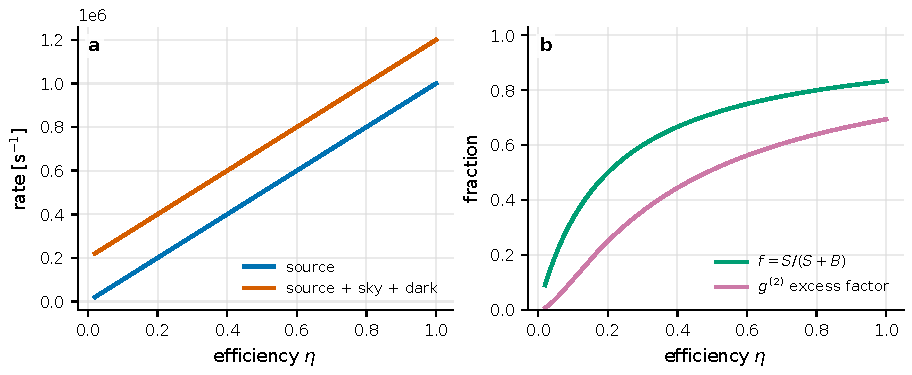
\includegraphics[width=0.85\linewidth]{figures/generated/chapter_03/ch03_detection_loss_background.pdf}
\caption{Two non-ideal effects that pull the observed statistics toward the Poisson baseline. Efficiency loss \(\eta\) is equivalent to the binomial thinning of a beamsplitter, randomly deleting photons and pressing the Mandel \(Q\) toward the zero point as \(Q\to\eta Q\) (but the normalized \(g^{(2)}(0)\) is unchanged); background dilution presses the source signal down by the square \(f^2\) of the source-photon fraction \(f\). Together with the multi-mode dilution \(1/M\), the two form the three gates by which astronomical intensity-correlation signals are pressed into a small-number excess.}
\label{fig:e07-detection-loss}
\end{figure}

\section{Chapter Summary}
\label{sec:e07-summary}

\begin{itemize}
  \item \textbf{Detection is absorption, so what is counted is normal-ordered.} The single-click rate \(\propto\langle\hat a^\dagger\hat a\rangle=\langle\hat n\rangle\); the two-coincident-click rate \(\propto\langle\hat a^\dagger\hat a^\dagger\hat a\hat a\rangle=\langle\hat n(\hat n-1)\rangle\). Using \([\hat a,\hat a^\dagger]=1\) one can prove exactly that \(\hat a^\dagger\hat a^\dagger\hat a\hat a=\hat n(\hat n-1)\).
  \item \textbf{\(n(n-1)\) rather than \(n^2\), because self-pairing is subtracted.} One START and one STOP must come from two \emph{different} absorptions; the \(N\) spurious pairs of ``the same photon paired with itself'' in \(N^2\) are automatically subtracted by normal ordering, leaving \(N(N-1)\) true pairs, precisely the origin of the \(b_2\) numerator of Chapter~\ref{chap:e06}.
  \item \textbf{Time gate + Mandel \(Q\).} Slice the event table into gates of width \(\Delta t\), count \(N\), obtain \(\bar N=r\Delta t\) and \(\sigma_N^2\); \(Q=(\sigma_N^2-\bar N)/\bar N\) takes Poisson as the zero point: \(Q=0\) Poisson, \(Q>0\) super-Poisson (thermal light), \(Q<0\) sub-Poisson (non-classical).
  \item \textbf{One identity connects the two languages.} From \(\langle N(N-1)\rangle=\sigma_N^2+\bar N^2-\bar N\) one derives \(g^{(2)}(0)=1+Q/\bar N\). When reporting, one must simultaneously give \(Q\), the gate width \(\Delta t\), the mode count \(M\), and the mean count \(\bar N\); none may be missing.
  \item \textbf{The \(1/M\) law of multi-mode dilution.} After averaging \(M\) independent thermal modes, \(\sigma_N^2=\bar N+\bar N^2/M\) and \(g^{(2)}(0)=1+1/M\). Polarization (2), spatial speckle, broadband multi-frequency modes, and gate width \(>\tau_c\) all contribute to \(M\), which is why the astronomical excess is often \(10^{-3}\) or \(10^{-6}\) rather than 1.
  \item \textbf{Detector non-idealities.} Efficiency \(\eta\) acts like a beamsplitter, binomial thinning pressing \(Q\to\eta Q\) (super-Poisson dragged toward Poisson), but the normalized \(g^{(2)}(0)\) unchanged; the background presses the signal down by \(f^2\); dead time/afterpulsing are left for Chapter~\ref{chap:e13}.
\end{itemize}

\medskip
\noindent\textbf{Questions to Ponder.}
\begin{enumerate}
  \item A beam of single-mode thermal light is measured to have \(g^{(2)}(0)=2\). If you widen the time gate from \(1\,\mathrm{ps}\) to \(1\,\mathrm{ns}\) (the coherence time still being \(1\,\mathrm{ps}\)), how many effective time modes does it become? To roughly what does \(g^{(2)}(0)-1\) then drop?
  \item If the detection efficiency \(\eta\) drops from \(0.5\) to \(0.05\), will the measured \(g^{(2)}(0)-1\) change? Will the Mandel \(Q\) change? Explain why for each.
  \item In an observation the source photons make up only \(f=1/3\) of the total count, the rest being sky-glow background. If the source itself is single-mode thermal light (\(g^{(2)}_{\rm src}(0)=2\)), roughly what \(g^{(2)}_{\rm obs}(0)\) do you measure in this channel?
\end{enumerate}
